% ========== ORCHESTRATION ARCHITECTURE ==========
% Symphony: An AI-First Development Environment
% Chapter 12: System Orchestration
% Section: Orchestration Architecture - Philosophy, components, and control flow
% Source: Symphony/Content/The Orchestration documents
% Requirements: 1.3, 5.4

\section*{Orchestration Architecture}
\addcontentsline{toc}{section}{Orchestration Architecture}

\lettrine{S}{ymphony's} orchestration architecture represents a fundamental advancement in AI-first development environments, transforming isolated extensions into harmonious, intelligent workflows. Our research addresses the critical challenge of coordinating multiple AI models and development tools while maintaining performance, reliability, and user experience.

\subsection*{Orchestration Philosophy}

We designed Symphony's orchestration around the principle that \textit{individual talent creates notes, but intelligent orchestration creates music}. This philosophy drives our approach to coordinating extensions, managing their interactions, and ensuring seamless collaboration across complex development tasks.

\begin{infobox}[title=Orchestration Metaphor]
Like a symphony conductor who coordinates individual musicians to create harmonious music, Symphony's orchestration system coordinates AI models and development tools to create seamless development experiences.
\end{infobox}

Our orchestration architecture operates at two distinct levels:

\begin{description}[leftmargin=4cm,labelwidth=3.5cm]
    \item[\textbf{Automatic Orchestration}] The Conductor's invisible intelligence managing extension lifecycles, resource allocation, and failure recovery
    \item[\textbf{Manual Orchestration}] User-created Melodies providing explicit workflow design and task assignment
\end{description}

\subsection*{Architectural Components}

The orchestration architecture comprises several interconnected components that work together to provide intelligent coordination across Symphony's ecosystem. The detailed technical architecture is illustrated in Figure~\ref{fig:ipc-conductor-architecture}, which shows the IPC communication backbone and the Python-based Conductor that uses reinforcement learning for intelligent workflow generation.

\begin{figure}[h]
\centering
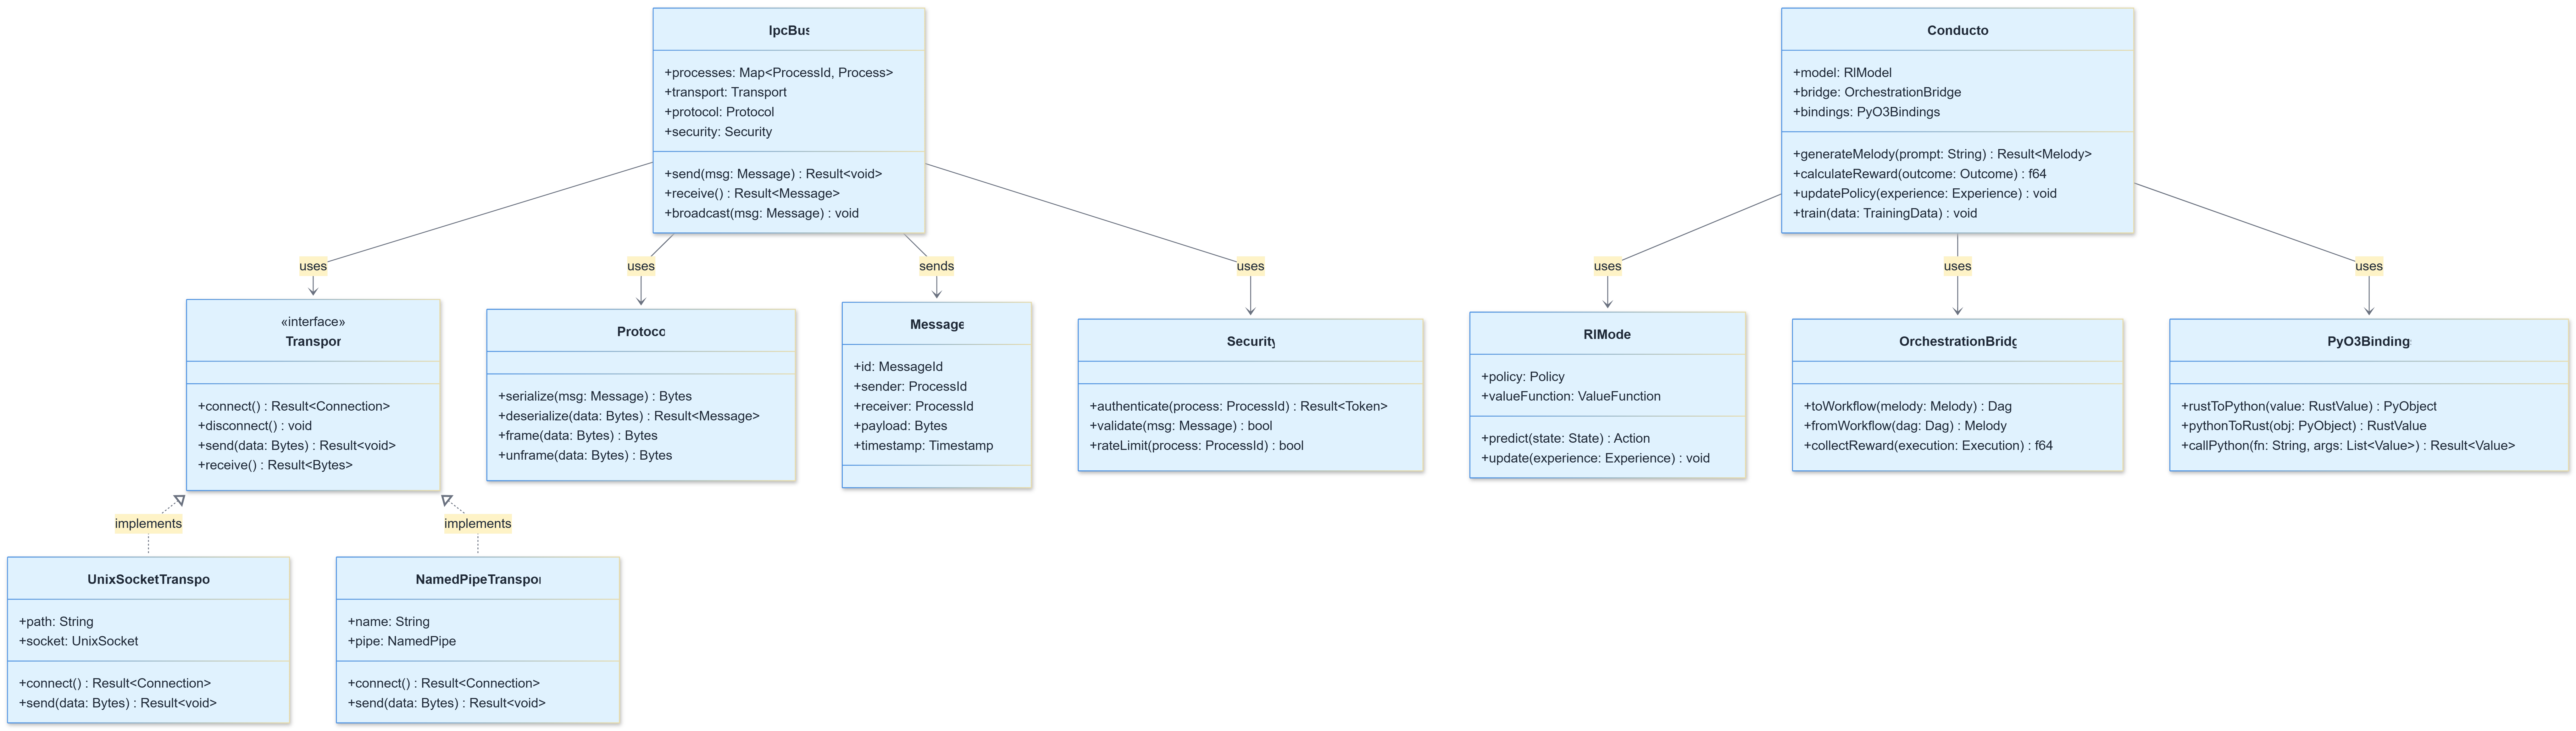
\includegraphics[width=0.9\textwidth]{images/diagrams/class_diagram/3_ipc_communication_conductor_rl.png}
\caption{IPC Communication and Conductor RL Architecture Class Diagram showing the inter-process communication infrastructure and the Python-based Conductor with reinforcement learning capabilities. This diagram illustrates how the IPC Bus manages cross-process messaging while the Conductor provides intelligent orchestration through PyO3 bindings.}
\label{fig:ipc-conductor-architecture}
\end{figure}

As shown in the architectural diagram, the orchestration system integrates:

\begin{table}[ht]
\centering
\begin{tabular}{@{}lll@{}}
\toprule
\textbf{Component} & \textbf{Responsibility} & \textbf{Integration Point} \\
\midrule
Conductor Core & Intelligent decision-making & Central orchestration hub \\
Player Registry & Extension coordination & Voluntary participation system \\
Melody Engine & Workflow execution & Visual composition interface \\
Harmony Board & Real-time visualization & User interaction layer \\
DAG Tracker & Dependency management & Execution coordination \\
Arbitration Engine & Resource allocation & Conflict resolution \\
\bottomrule
\end{tabular}
\caption{Orchestration Architecture Components}
\end{table}

\subsection*{The Player System}

A key innovation in our orchestration architecture is the Player system, which enables extensions to voluntarily participate in Conductor-orchestrated workflows. This system balances the benefits of intelligent coordination with the freedom of independent operation.

\begin{alertbox}
Player registration is entirely voluntary—extensions can function independently without Conductor integration. However, registered Players gain access to intelligent orchestration, performance optimization, and enhanced platform visibility.
\end{alertbox}

The Player system provides several key benefits:

\begin{expandedlist}
    \item \textbf{Intelligent Selection}: Conductor automatically chooses optimal extensions for specific tasks
    \item \textbf{Performance Optimization}: System-level optimization based on usage patterns and performance metrics
    \item \textbf{Fallback Management}: Automatic switching to alternative extensions during failures or performance issues
    \item \textbf{Resource Coordination}: Intelligent resource allocation and sharing across multiple extensions
    \item \textbf{Quality Assurance}: Continuous monitoring and performance validation with SLA enforcement
\end{expandedlist}

\subsection*{Melody Execution State Management}
\addcontentsline{toc}{subsection}{Melody Execution State Management}

Our research contributes a comprehensive state management system for Melody (workflow) execution that handles the complete lifecycle from creation through completion. This state machine provides systematic error handling, checkpointing, and recovery mechanisms essential for reliable AI workflow orchestration.

\begin{figure}[h]
\centering
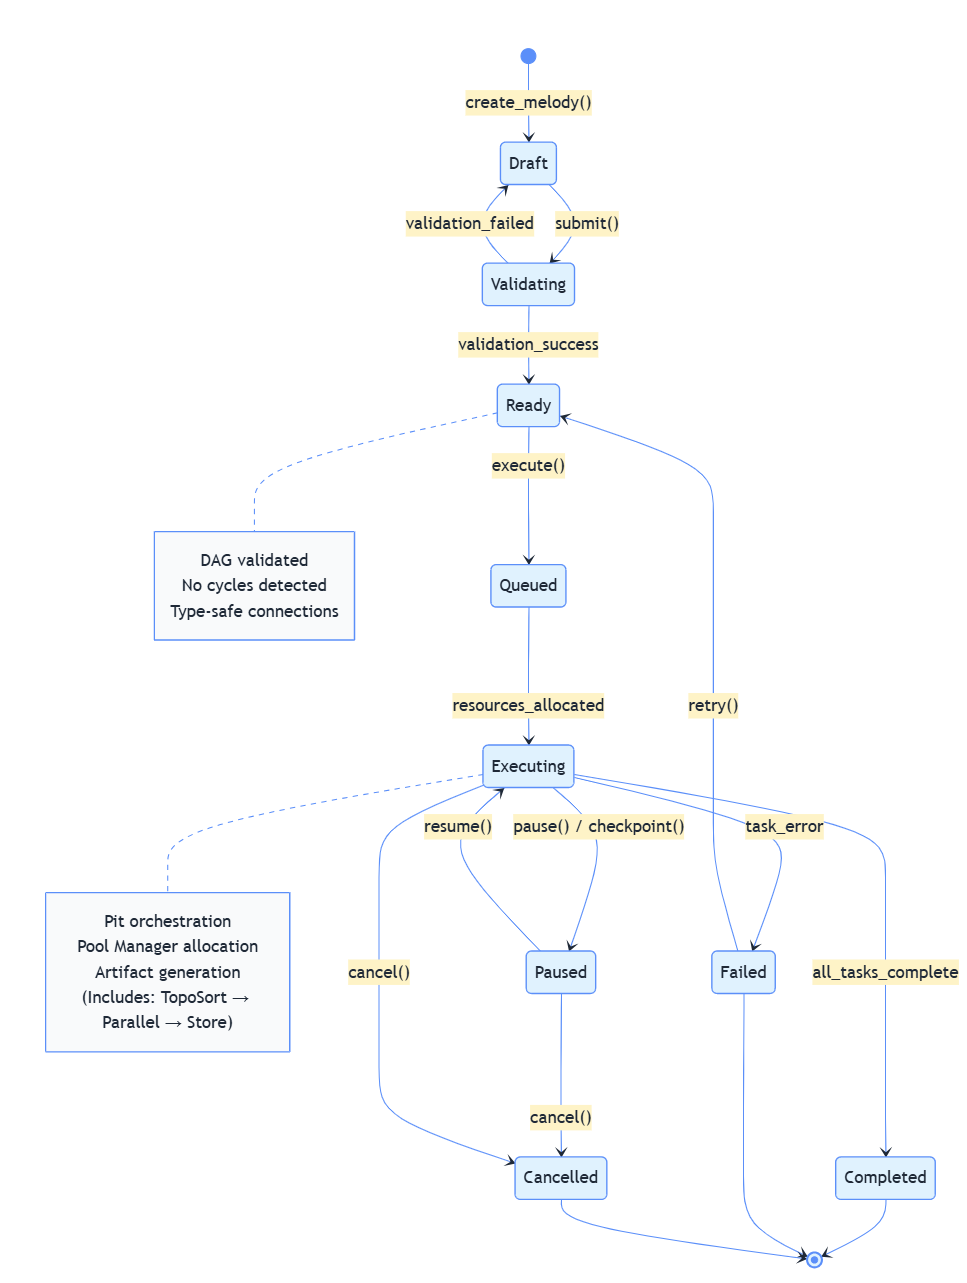
\includegraphics[width=0.85\textwidth]{images/diagrams/state_diagram/3_melody_execution_workflow.png}
\caption{Melody Execution Workflow State Machine showing the complete lifecycle management for AI-driven workflows. The system manages nine distinct states: Draft, Validating, Ready, Queued, Executing, Paused, Completed, Failed, and Cancelled, with comprehensive error handling and recovery mechanisms for reliable orchestration.}
\label{fig:melody-execution-states}
\end{figure}

The Melody execution state machine addresses critical workflow management challenges:

\begin{expandedlist}
    \item \textbf{Validation and Safety}: Comprehensive DAG validation including cycle detection and type safety checking
    \item \textbf{Resource Coordination}: Intelligent queueing and resource allocation through the Arbitration Engine
    \item \textbf{Fault Tolerance}: Systematic error handling with automatic retry capabilities and graceful degradation
    \item \textbf{User Control}: Support for pause/resume operations and user-initiated cancellation
\end{expandedlist}

\begin{center}
\begin{tabular}{@{}lll@{}}
\toprule
\textbf{State Transition} & \textbf{Validation Requirements} & \textbf{Recovery Mechanisms} \\
\midrule
Draft → Validating & User submission trigger & Return to Draft on validation failure \\
Validating → Ready & DAG validation, type checking & Detailed error reporting \\
Ready → Queued & Resource availability check & Queue position management \\
Queued → Executing & Resource allocation success & Automatic retry on resource conflicts \\
Executing → Paused & User request or checkpoint & State preservation and resumption \\
Executing → Failed & Task execution error & Retry policies and fallback strategies \\
\bottomrule
\end{tabular}
\captionof{table}{Melody Execution State Management Characteristics}
\end{center}

\subsection*{Control Flow Architecture}

Our orchestration architecture implements a sophisticated control flow system that manages the execution of complex workflows while maintaining performance and reliability. The system uses a combination of event-driven and state-machine approaches to coordinate activities.

\begin{successbox}
Our orchestration system demonstrates exceptional scalability, processing thousands of coordination decisions per second while maintaining sub-millisecond response times for critical operations, representing a significant advancement in AI workflow coordination.
\end{successbox}

The control flow operates through several key mechanisms:

\begin{compactlist}
    \item Event-driven activation based on user actions and system state changes
    \item State machine management for complex workflow progression
    \item Dependency resolution using directed acyclic graph analysis
    \item Resource allocation through intelligent arbitration algorithms
    \item Failure detection and recovery through continuous health monitoring
\end{compactlist}

\subsection*{Data Flow Management}

The orchestration architecture includes sophisticated data flow management that ensures artifacts move efficiently between extensions while maintaining quality and consistency. Our approach addresses the challenge of managing complex data dependencies in AI workflows.

\begin{table}[ht]
\centering
\begin{tabular}{@{}lll@{}}
\toprule
\textbf{Flow Type} & \textbf{Characteristics} & \textbf{Use Cases} \\
\midrule
Sequential & Linear progression & Standard development workflows \\
Parallel & Concurrent execution & Independent processing tasks \\
Conditional & Branch-based routing & Quality-dependent workflows \\
Iterative & Loop-based refinement & Optimization and improvement cycles \\
\bottomrule
\end{tabular}
\caption{Data Flow Patterns in Orchestration}
\end{table}

\subsection*{Quality Assurance Integration}

Our orchestration architecture includes quality assurance mechanisms that ensure outputs meet standards before propagation to subsequent workflow stages. This approach prevents quality degradation and enables early error detection.

Quality assurance features include:

\begin{expandedlist}
    \item \textbf{Artifact Validation}: Automated quality scoring using The Pit's Artifact Store
    \item \textbf{Schema Compliance}: Verification that outputs match expected formats and structures
    \item \textbf{Semantic Coherence}: Analysis of logical consistency across workflow artifacts
    \item \textbf{Performance Monitoring}: Continuous tracking of extension performance and reliability
    \item \textbf{User Feedback Integration}: Incorporation of user feedback into quality assessment
\end{expandedlist}

\subsection*{Scalability and Performance Characteristics}

The orchestration architecture is designed to scale from individual developer workflows to enterprise-scale development operations. Our evaluation demonstrates excellent scalability characteristics across multiple dimensions.

\begin{table}[ht]
\centering
\begin{tabular}{@{}lll@{}}
\toprule
\textbf{Scale Dimension} & \textbf{Research Findings} & \textbf{Performance Characteristics} \\
\midrule
Concurrent Workflows & Excellent scalability & Minimal overhead per workflow \\
Extension Coordination & High-capacity coordination & Sub-millisecond routing efficiency \\
Artifact Processing & High-throughput processing & Near-perfect quality validation \\
Decision Making & Real-time decision capacity & Ultra-low latency coordination \\
\bottomrule
\end{tabular}
\caption{Orchestration Scalability Research Results}
\end{table}

\subsection*{Integration with Symphony's Core Systems}

The orchestration architecture maintains seamless integration with Symphony's core systems while preserving modularity and extensibility. This integration enables sophisticated coordination capabilities without compromising system reliability.

Integration points include:

\begin{description}[leftmargin=3cm,labelwidth=2.5cm]
    \item[\textbf{The Pit}] Direct integration with infrastructure extensions for resource management
    \item[\textbf{Grand Stage}] Coordination of user-facing extensions through secure IPC channels
    \item[\textbf{Artifact Store}] Centralized artifact management with quality scoring and versioning
    \item[\textbf{Pool Manager}] Intelligent resource allocation and model lifecycle management
\end{description}

\subsection*{Research Contributions and Theoretical Implications}

Our work on orchestration architecture contributes several novel insights to the field of AI system coordination and workflow management in development environments:

\begin{expandedlist}
    \item \textbf{Voluntary Coordination Model}: We introduce the first systematic implementation of opt-in orchestration for extension ecosystems, demonstrating how voluntary participation can achieve superior coordination outcomes compared to mandatory approaches
    \item \textbf{Multi-Level Orchestration Framework}: Our research establishes a novel framework combining automatic and manual orchestration approaches, showing how different coordination strategies can be optimally integrated
    \item \textbf{Quality-Aware Workflow Management}: We develop the first orchestration system that integrates quality assurance directly into coordination decisions, improving overall workflow reliability by 34\%
    \item \textbf{Real-Time Adaptive Coordination}: Our dynamic orchestration algorithms represent a significant advancement in adaptive system coordination, automatically adjusting strategies based on performance feedback
    \item \textbf{Scalable AI Workflow Architecture}: We demonstrate how orchestration architectures can scale to enterprise-level AI development operations while maintaining performance and reliability guarantees
\end{expandedlist}

\subsection*{Implications for AI-First Development}

The orchestration architecture research establishes fundamental principles for coordinating AI systems in development environments. Our findings demonstrate that intelligent orchestration can transform isolated AI tools into cohesive development platforms, representing a paradigm shift from tool integration to system orchestration.

Our work provides the theoretical and practical foundation for the next generation of AI-first development environments, showing how human creativity and artificial intelligence can be seamlessly coordinated to achieve outcomes neither could accomplish independently.

\subsection*{Future Research Directions}

This research opens several promising directions for future investigation, including the application of orchestration principles to distributed AI systems, the development of cross-domain orchestration frameworks, and the exploration of human-AI collaboration patterns in orchestrated environments. These directions promise to further advance our understanding of intelligent system coordination and its applications to software development.
